%
% fig-randkarten.tex
%
% (c) 2025 Prof Dr Andreas Müller
%
\begin{figure}
\centering
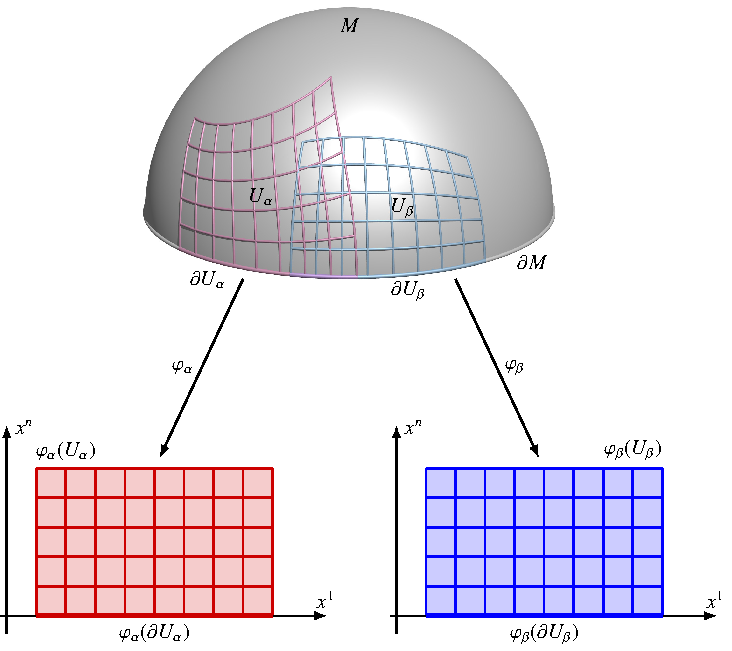
\includegraphics{chapters/040-green/images/randkarten.pdf}
\caption{Eine Mannigfaltigkeit mit Rand hat Karten, die eine offene
Teilmenge von $\{x^n=0\}$ als Rand enthalten.
Kartenwechsel sind beliebig oft differenzierbare Abbildungen, die
Randteile in Randteile abbilden (ausgezogene Linien entlang der
Hyperebene $\{x^n=0\}$).
\label{buch:green:green:fig:randkarten}}
\end{figure}
